\chapter{Methods and Characterisation}

\section{Optical CT Materials and Methods}
\subsection{Hardware}

Our  optical CT system is area-detector based, allowing for fast 3-D scanning. A high quality scientific Complementary Metal-Oxide Semiconductor (CMOS) camera (Zyla sCMOS, Andor Technology PLC, Belfast, UK) has excellent sensitivity, read-out noise and fast read-out speed. 

We have two illumination sources. A flat-panel red Light Emitting Diode (LED) 
(PHLOX-LEDR-BL-100x100-S-Q-1R-24V, Phlox, Aix-en-Provence, France), with a wavelength of 633nm provides uniform lighting appropriate for imaging PRESAGE\texttrademark , a radiochromic plastic which has a strong absorption peak at 632nm. 
For tissue imaging the wavelength most appropriate for each sample is provided through the use of a  new broadband white light source (SugarCUBE LED Illuminator, Nathaniel Group Inc., VT, USA) and tunable filter (VariSpec, PerkinElmer, Inc., MA, USA). 

	\begin{figure}[H]
		\centering
		\subfigure[System setup diagram]{\label{subfig:setupdia}
			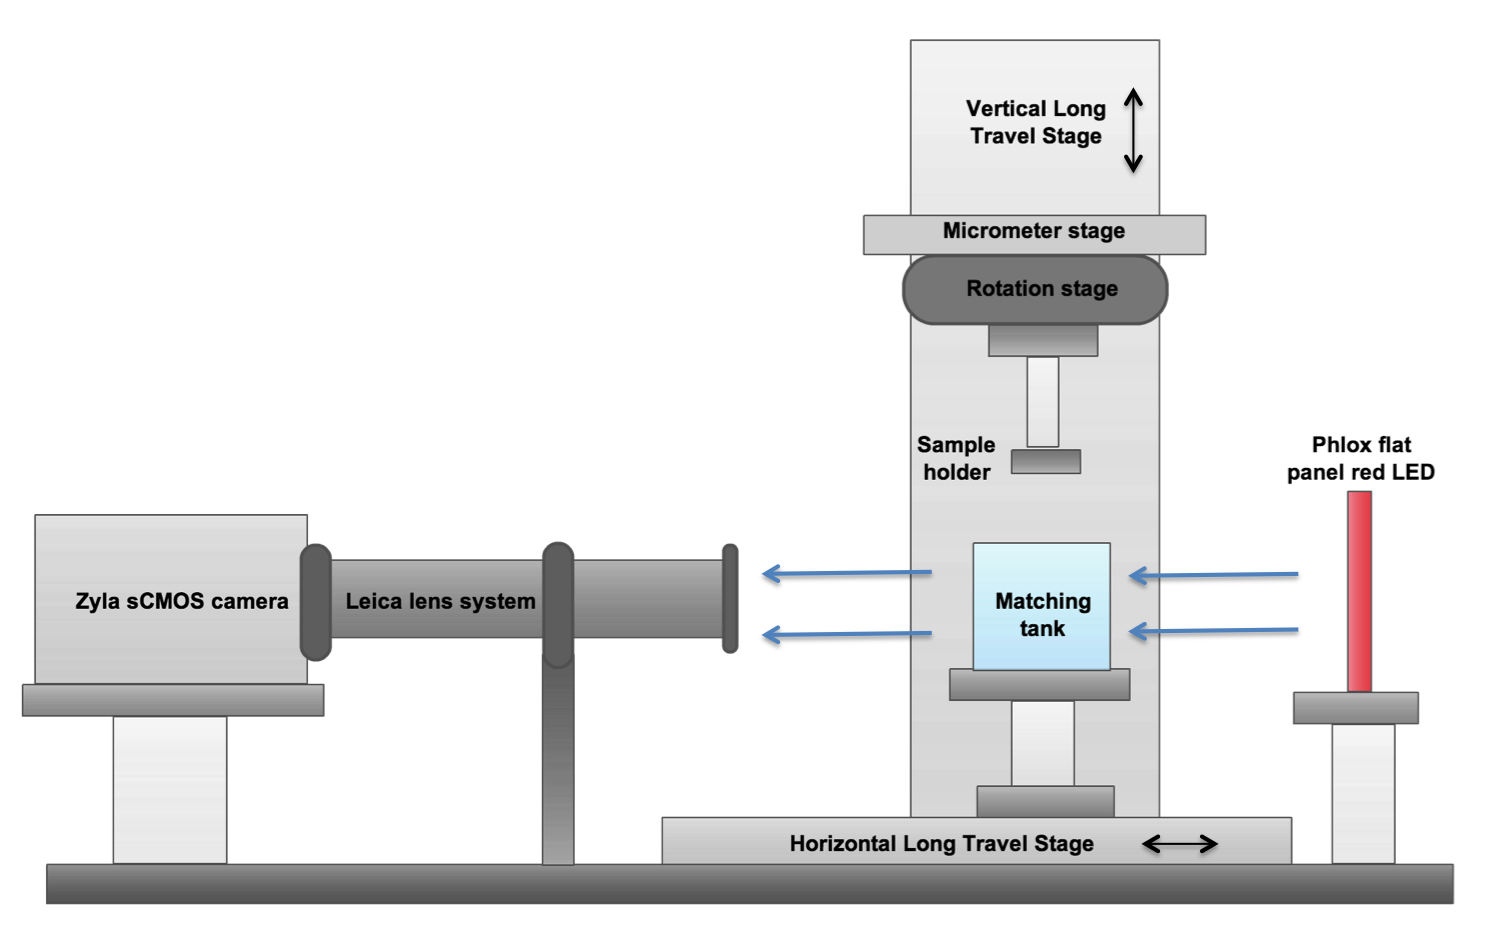
\includegraphics[width = \textwidth]{meth_img/setup_diagram.png}}
		\subfigure[System setup photo]{\label{subfig:setupphoto}
			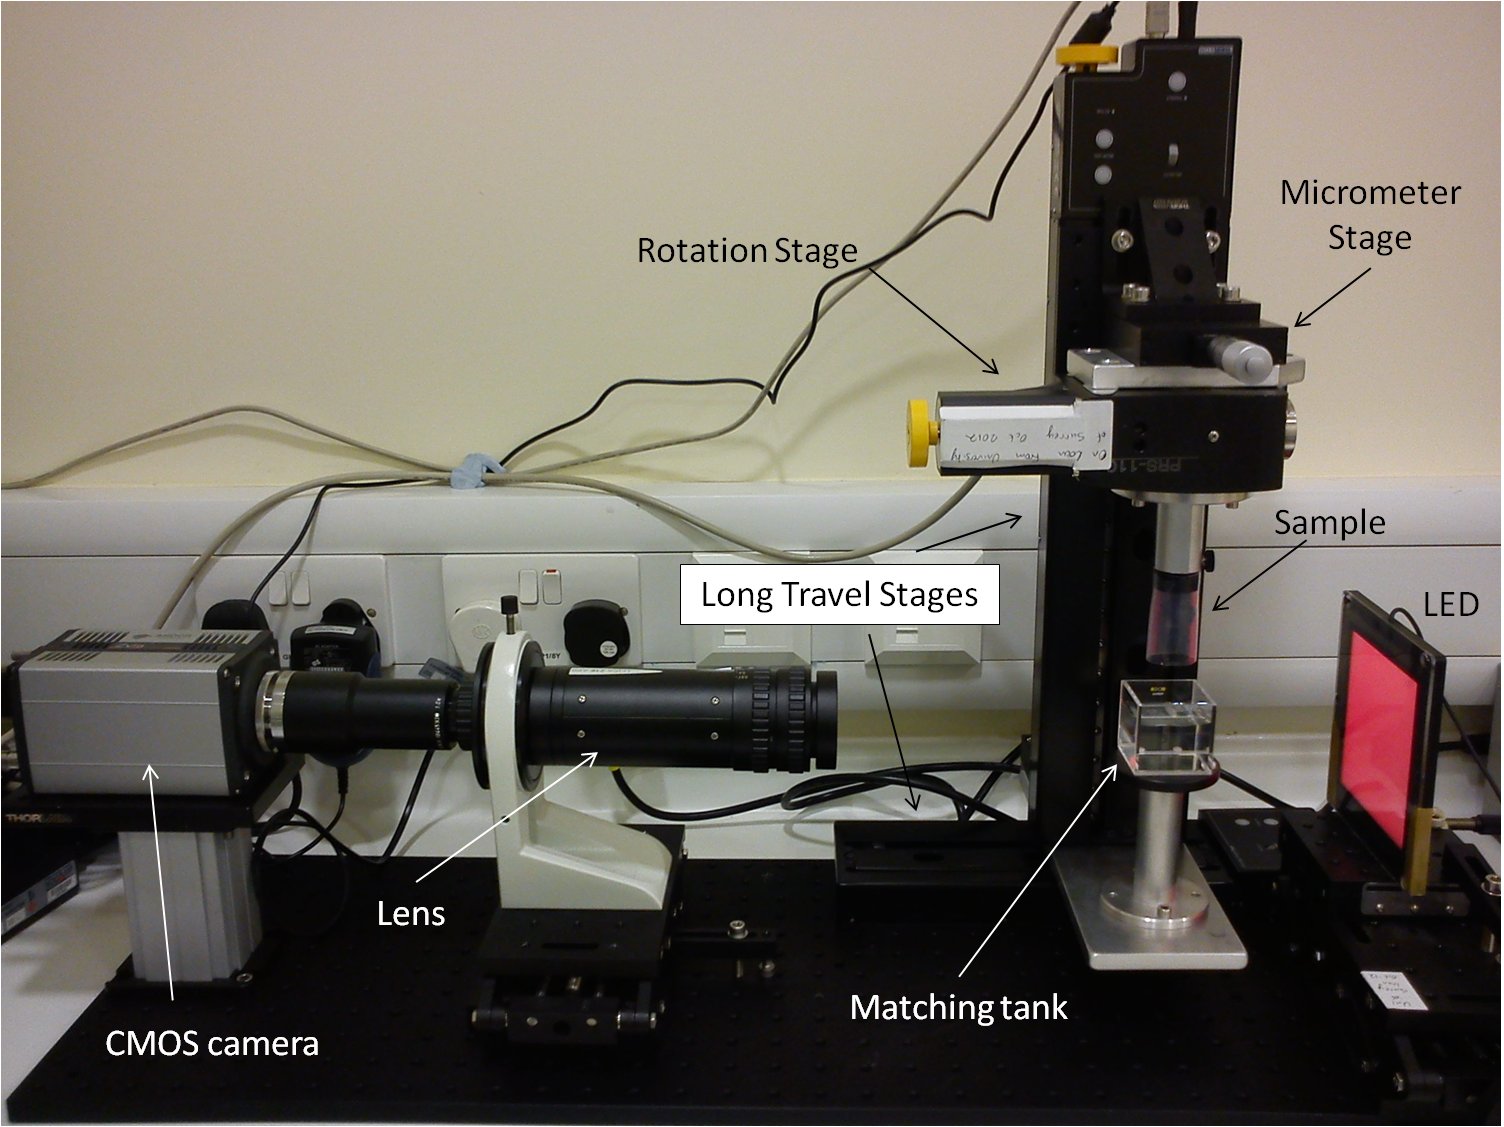
\includegraphics[width = 0.85\textwidth]{meth_img/Tidy_setup.png}}
		\caption{Diagram and picture  of current set-up of optical CT system at the ICR with principal parts of apparatus labelled.}
		\label{fig:setup_pic}
	\end{figure}

Samples are suspended from a rotary stage (PRS-110 ZSS43, PI miCos GmbH, Eschbach, Germany) in a glass matching tank (Part 704-002-40-10, Hellma GmbH, M\"{u}llheim, Germany). The COR can be adjusted through a micrometer stage which moves the rotation stage. A COR-checker LabView program checks for accurate alignment of the COR with the centre of the FOV. Off-centre COR leads to artefacts which can be corrected as part of the reconstruction.

The matching tank is filled with `matching liquid' with an RI close to that of the sample, avoiding refraction at the curved surface of the sample. For PRESAGE samples this matching fluid was a solution of (97\% ethyl hexyl salicylate and 3\% 4-methoxycinnamic acid 2-ethylhexyl ester) giving the same refractive index as the PRESAGE\textregistered. The clearing solution used for each tissue sample was used for matching fluid.

For initial measurements  the rotation stage was supported on a large optical post. In an updated system this post was replaced with an Integrated Long Travel Stage (LTS-300/M, Thorlabs Ltd., Ely, UK ) which allows  accurate and reproducible vertical positioning of samples. 
In collaboration with the ICR workshop, a novel mounting system has been developed to give reproducible positioning of samples allowing pre and post-irradiation scans of dosimetry gel. 
Two custom sample mounts are used for dosimetry and tissue samples respectively. The dosimetry mount fits caps that are fixed to PRESAGE samples, meaning the samples are in the same orientation for every scan. The tissue mount has two additional stages, giving the flexibility to position irregular samples on the COR independently of moving the COR.  

An additional Long Travel Stage (LTS-150/M, Thorlabs LTD., Ely, UK ) allows accurate positioning of the sample and tank along the optical axis.  

Light is collected by an imaging lens system made up of  components of the modular `Z16 APO' zoom system  (Leica Microsystems GmbH, Wetzlar, Germany, see \cite{Doran:2010hn} for details). The use of the zoom lens allows manual adjustment of the focus and magnification. However, in general the manual focus is left constant and we use the LTS stage to move the sample and tank along the optical axis for focusing - more repeatable. Add focusing protocol.








\subsection{Software}
\subsubsection{Acquisition}

Image acquisition and rotation are controlled synchronously  by PC using an in-house program written in LabView (National Instruments Corporation Ltd., Berkshire, UK). The high capacity of the PC and camera allows for fast read-out of images giving much reduced scan times to others previously reported. For standard scans  images are acquired during continuous rotation of the sample. 

If projections are acquired with no binning then a Step-and-shoot method with averaging of several projections is used to improve the SNR. This method takes much longer.

Include algorithms? Maybe in appendix?




\subsubsection{Reconstruction}
Reconstruction is carried out via Filtered Back-projection (FBP) incorporating a `correction scan' using in-house software  written by  SJD in IDL (Excelis Visual Information Solutions, Boulder, CO) (see \cite{doranestablishing2013}). 
%Shepp-Logan filter used?




`Dark' field (DF) and `light' field (LF) images correct for structural noise in the camera and non-uniformities in the light path respectively. In general 30 DF (with cap on camera) and LF (no sample present) images were averaged for each scan and images are corrected during reconstruction according to  equation (4) of Krstaji\'{c} \cite{Krstajic:2007ec}.  

The software also allows for adjustment to correct for off-axis  centre of rotation (COR). In the updated system  the rotation stage is mounted on a micrometer stage allowing more precise alignment of the CoR. If the CoR is not aligned with the central pixel column then the sample will appear to drift across the screen and projection data will not be consistent for all angles. \cite{Oldham:2006b}

A ring artefact correction has been added to the reconstruction, based on [INSERT reference]. The number of pixels can be chosen depending on the matrix size of the projections.


\subsection{Dosimetry protocol}


Optical CT imaging of PRESAGE samples was carried out in two modes.
For qualitative visualisation of irradiation patterns fast scans were used, while samples for PVDR assessment were scanned with high-resolution scans. All scans had an aperture setting of A=1 so that the DOF encompassed the entire sample.


		
	\begin{table}[H]
		\centering
		\begin{tabular}{ p{2.3cm}  p{2.5cm} p{2.5cm}  p{2.3cm} p{2.5cm}  }
			\hline
			\textbf{Scan} & \textbf{Projections} &\textbf{Pixels}   &\textbf{Voxel size ($\mu$m)} & \textbf{Acquisition time} \\ \hline 
			Fast  & 1000 & $512\times 512$  & 20.8 &2.5 minutes \\ %\hline
			High-resolution & 3200 & $2048\times 2048$ &  5.2 & 1 hour \\ 
			\hline
		\end{tabular}
		\caption{Different scanning parameters for MRT}
		\label{table:scansettings}
	\end{table}
	
	
	

	\begin{figure}[H]
		\centering
		\subfigure[Projection 190]{\label{subfig:presageproj1}
			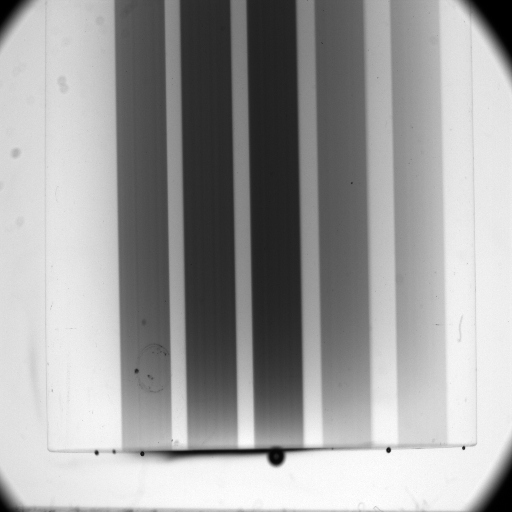
\includegraphics[width=0.45\textwidth]{meth_img/P19_proj_190.jpeg}}
		\subfigure[Projection 690]{\label{subfig:presageproj2}
			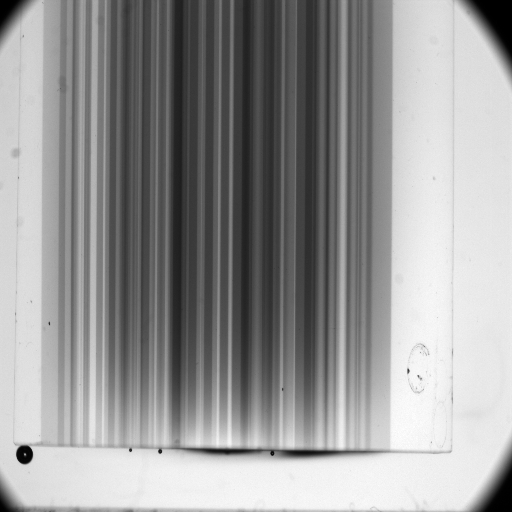
\includegraphics[width=0.45\textwidth]{meth_img/P19_proj_690.jpeg}}
		\caption{Projections taken $180^{\circ}$ apart through a PRESAGE\texttrademark ~sample irradiated at the ESRF with a defined test pattern of known line widths. Some air bubbles can be seen as dark circles at the base of the sample. Faint marks in the upper left parts of the images are caused by dust in the optics which will be corrected by a Light Field scan. In \ref{subfig:presageproj2} a mark on the side of the sample itself can be seen near the bottom right. A small refractive index mismatch between the sample and liquid is seen by the faint outline of the sample walls. This will result in a circular artefact in reconstructed slices.  }
		\label{fig:presage_projections}
	\end{figure}



Projections, such as those seen in Figure ~\ref{fig:presage_projections} were reconstructed to give slices through the sample. A view through the sample made up of 20 averaged slices is seen in Figure~\ref{fig:presage_slice}. It was possible to average slices and thereby improve the SNR of the image because the sample was axially uniform. A clear dose pattern can be seen in the sample, similar to those previously reported by Doran \textit{et al.} \cite{doranestablishing2013}. Some blurring and ring artefacts can be seen but the overall  image quality is good with high SNR. The RI mismatch artefact is not significant but could be improved. Lineprofiles for each row numbered on the slice are shown in Figure~\ref{fig:P19_lp} showing how the system response falls off with increasing line-pairs per mm (lppm).  A rolling baseline as previously reported by Doran is seen for line 3 whereby the signal falls off towards the edges of the sample.  The highest lppm pattern resolved was 20 lppm, seen  on the far left of line 4. Three patterns on line 4 were not resolved representing 30, 40 and 50 lppm. This means the smallest resolvable object was between 66-$100\mu m$ and not  $40\mu m$ as predicted by the MTF data. This discrepancy is probably due a combination of blurring due to reconstruction, imperfect focusing and the fact that projections of the patterns are not always acquired with the pattern in the centre of the focal plane.  
The results from this phantom verified the optical CT system was working for dosimetry, allowing us to move onto adapting the system for imaging tissue. 



	\begin{figure}[H]
		\centering
		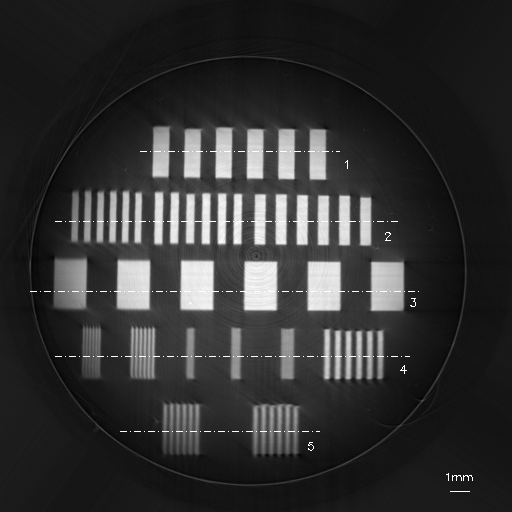
\includegraphics[width=0.72\textwidth]{meth_img/P19_recon370-399av_lineprofiles.png}
		\caption{Reconstructed slice of the PRESAGE\texttrademark ~sample seen in Fig.~\ref{fig:presage_projections}. The image is a result of 20 averaged slices to improve the SNR. Annotations refer to line profiles plotted in Fig.~\ref{fig:P19_lp}. }
		\label{fig:presage_slice}
	\end{figure}
	
	\begin{figure}[H]
		\centering
		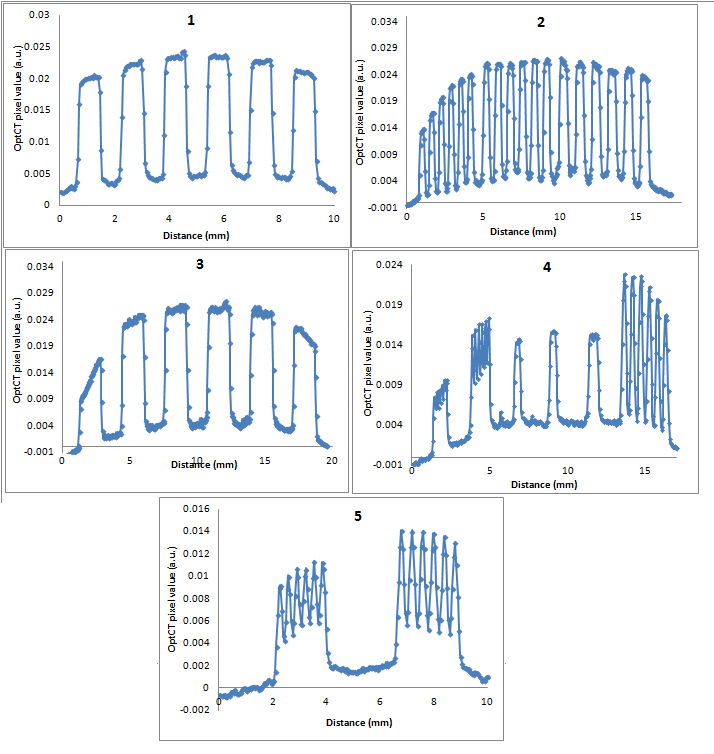
\includegraphics[width=\textwidth]{meth_img/P19_lineprofiles.png}
		\caption{Lineprofiles for PRESAGE\texttrademark ~sample shown in Figure~\ref{fig:presage_slice}. The highest resolution pattern resolved was 20 lppm (far left of pattern 4) but  the 30, 40 and 50 lpppm patterns on line 4 are unresolved. No modulation is seen for these patterns indicating that objects smaller than $100\mu m$ cannot be imaged.}
		\label{fig:P19_lp}
	\end{figure}




\subsection{Tissue imaging protocol}



Before imaging, tissue samples must undergo a series of preparation steps:
\begin{itemize}
	\item Fix in $70\%$ ethanol in phosphate-buffered saline (PBS) overnight
	\item Embed in $0.75\%$ agarose for stability
	\item $3-4$ washes of $100\%$ ethanol
	\item Washes of $30\%$ and $70\%$ 1:2 benzyl benzoate:benzyl alcohol (BABB) in ethanol
	\item $1-2$ washes of $100\%$ 1:2 BABB (refractive index 1.559)
	\item Superglue agarose to sample holder prior to imaging with 1:2 BABB matching fluid.
\end{itemize}



Due to the small size and irregular shapes of tissue samples, a new positioning system was necessary to allow flexible positioning of samples on the centre of rotation. This is coupled with a LabView program for alignment makes sample positioning much easier, previously difficult and time consuming. 




	\begin{figure}[H]
		\centering
		%	\subfigure[Clearing heart]{\label{subfig:clearingheart}
		%		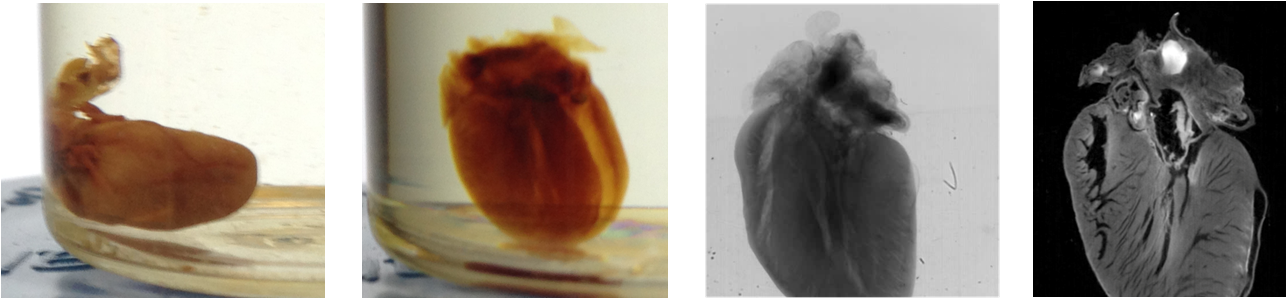
\includegraphics[width = \textwidth]{clearing_process_heart.png}}
		%	\subfigure[Clearing brain]{\label{subfig:clearingbrain}
		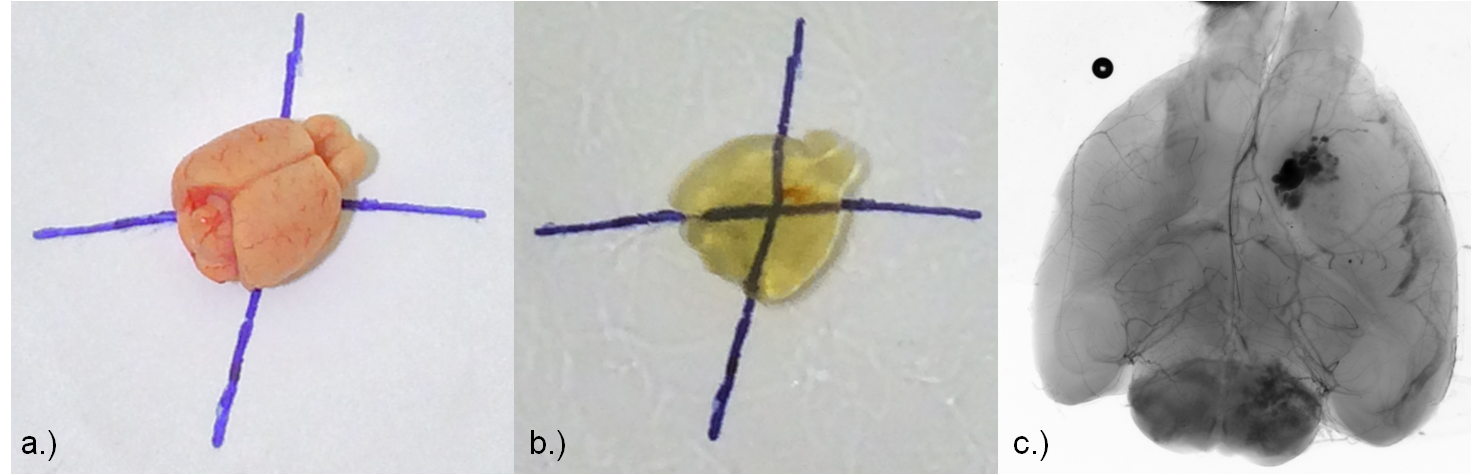
\includegraphics[width = \textwidth]{meth_img/Brain_J5_clearing.png}
		\caption{a.) Example of an uncleared mouse brain, b.) a cleared mouse brain in 1:2 BABB solution, c.) a projection image of the cleared brain mounted in the optical CT system.}
		\label{fig:clearing}
	\end{figure}




%\begin{figure}[H]
%	\centering
%	\subfigure[System setup photo]{\label{subfig:tissuesetupphoto}
%		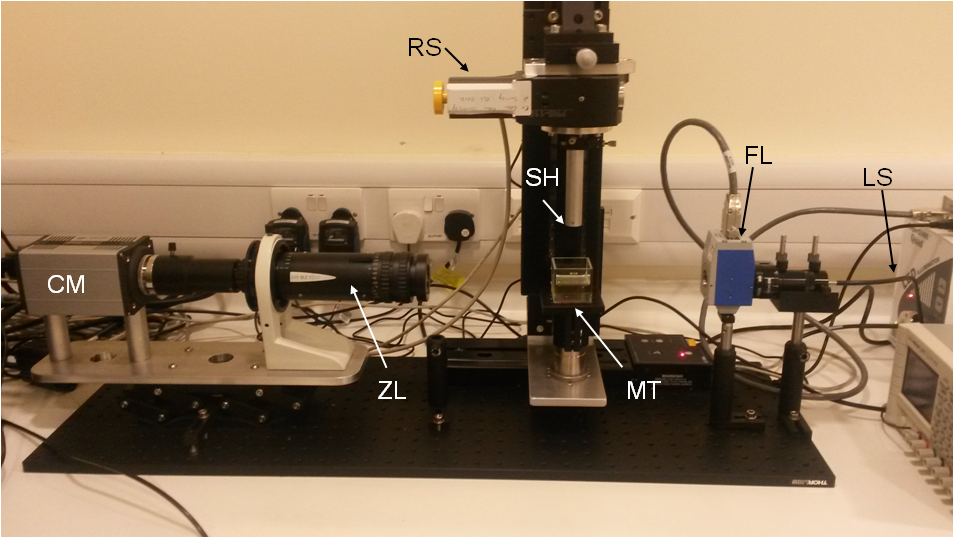
\includegraphics[width = 0.85\textwidth]{Tissue_set-up.png}}
%	\caption{Diagram and picture  of current set-up of tissue OptCT system at the ICR with principal parts of apparatus labelled. Add pictures of sample preparation.}
%	\label{fig:tissuesetup_pic}
%\end{figure}



Examples images of different healthy rodent organs are shown in Figure~\ref{fig:heart_brain}. Clearing with BABB has worked well and all contrast is endogenous. Clearing reduces light attenuation due to scattering, so any contrast is due to natural differences in light absorption properties between different tissue types. Highly attenuating areas, such as haemoglobin in the heart, or lipid-dense areas of the brain, are bright in these optical CT absorption scans.

Images of tissues containing tumours are shown in Figure~\ref{fig:tumours}, ranging from a large neuroblastoma tumour, of the order of 10mm, to a tumour cell spheroid around $100\mu$m diameter, at the extreme resolution limit of the system. It was noted that large and highly attenuating tissues (such as neuroblastoma tumours) required longer clearing time.


	\begin{figure}[H]
		\centering
		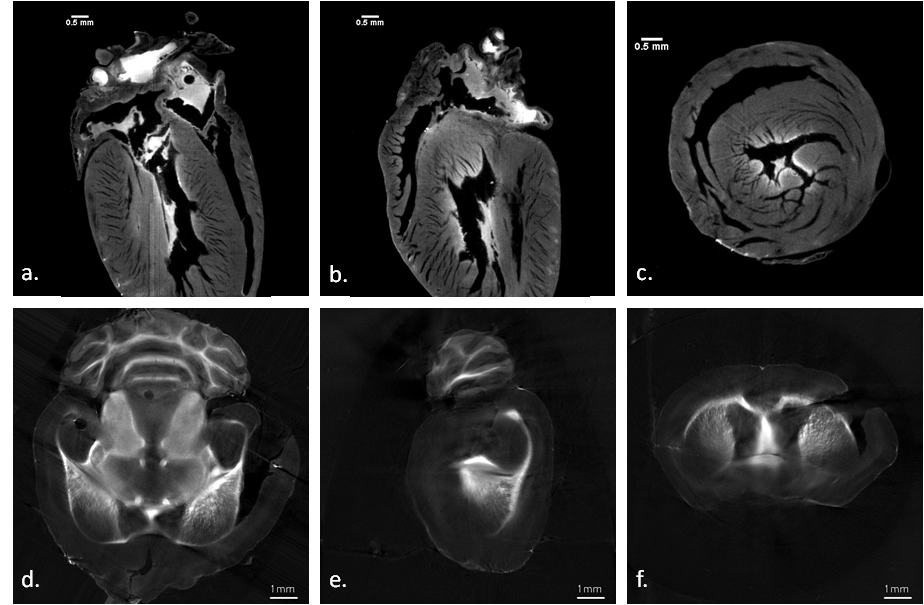
\includegraphics[width = \textwidth]{meth_img/heart_brain_sclbr.png}
		\caption{a-c.) Orthogonal slices of a reconstructed image volume of a mouse heart with endogenous contrast, most likely due to the presence of haemoglobin. d-f.) Orthogonal slices of a reconstructed image volume of a mouse brain where bright areas are likely due to attenuation due to lipid content of the brain. These images demonstrate high-resolution, highly detailed data reconstructed from absorption optical CT scans,  without addition of external contrast.}
		\label{fig:heart_brain}
	\end{figure}
	
	\begin{figure}[H]
		\centering
		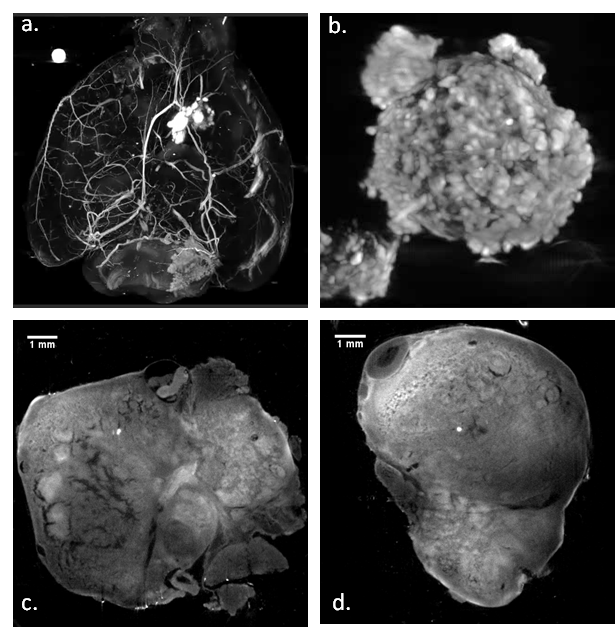
\includegraphics[width = \textwidth]{meth_img/tumours.png}
		\caption{a.) Maximum intensity projection (MIP) of a mouse brain with an orthotopic glioblastoma tumour. A highly attenuating artefact due to an air bubble is seen in the top left corner. The mouse was injected with Evans Blue, an absorbing permeability marker which has stained the vasculature. The tumour was rich in haemoglobin and also appears very attenuating. This shows the potential for optical CT imaging of vasculature. b.) MIP image of a tumour cell spheroid stained with haematoxylin. c-d.) Orthogonal slices through a neuroblastoma tumour showing the detail possible using an anatomical scan. Additional functional information can be added with the use of fluorescent markers. }
		\label{fig:tumours}
	\end{figure}









\section{Optical CT system characterisation}

\subsection{Linear response}

In order to establish the relationship between optical CT reconstructed pixel value and optical absorbance,  gel finger phantoms were made in a similar fashion to \cite{Oldham:2003}.  

10\% porcine gelatin (Sigma, REF) was made in water. Add exact method? Maybe in appendix. Heat to 60?deg, vacuum, stir while cooling to 25?. 

A specialised finger phantom mould was made by the ICR workshop. A 3-D printed holder contained slots to hold metal rods on one side and can be attached directly to the rotation stage on the other. A cylinder of Teflon FEP heat-shrink plastic (Holscot Fluoroplastics Limited, Grantham, UK) was used to provide support for the gelatin. Teflon FEP has an RI of 1.341  making it a very close match for water and gelatin. \cite{Krstajic:2006kna} Cylindrical pieces of Teflon sleeving were cut a length of 4cm, the height of the matching tank and one end was heat shrunk onto the plastic mould providing a secure support for the cooling gelatin. It was important to make sure the Teflon sleeving was not too tight around the plastic mould, if no air can come through the bottom then the metal rods cannot be removed easily creating air-bubbles leading to attenuation artefacts. Three removable metal rods were placed in each mould.


Clear gelatin was allowed to set at room temperature around the metal rods, which  were then carefully removed.  Evans Blue (T-1824), an azo dye which is both optically absorbing and  fluorescent, was used to provide optical contrast. Small amounts of Evans blue were added progressively to gelatin which was kept at 30deg using a heater-stirrer. The Evans blue doped gelatin was injected into the inclusions left by the metal rods using a 1ml syringe. A cuvette of each concentration of Evans blue gelatin  was filled and allowed to set. The optical absorbance of each cuvette was measured using a spectrophotometer (REF). Phantom A had 3mm diameter inclusions and phantom B, 2mm inclusions, with increasing Evans Blue concentrations.

The phantoms were scanned under the same imaging conditions. The matching liquid used was 4.5\% salt solution (RI $\approx 1.341$) which  gives a closer refractive index match than water. The average reconstructed pixel value of each finger was calculated from a single axial slice and averaged over a $25 \times 25$ pixel area within the inclusion (see Figure~\ref{fig:fingerphantoms_roi_EB}b).
As can be seen in Figure~\ref{fig:fingerphantoms_roi_EB}c, the reconstructed pixel value of the optical CT system is linearly related to the optical absorbance as measured by  spectrophotometer.   The use of two phantoms verifies the linear relationship and the repeatability of measurements.  

	\begin{figure}[H]
		\centering
		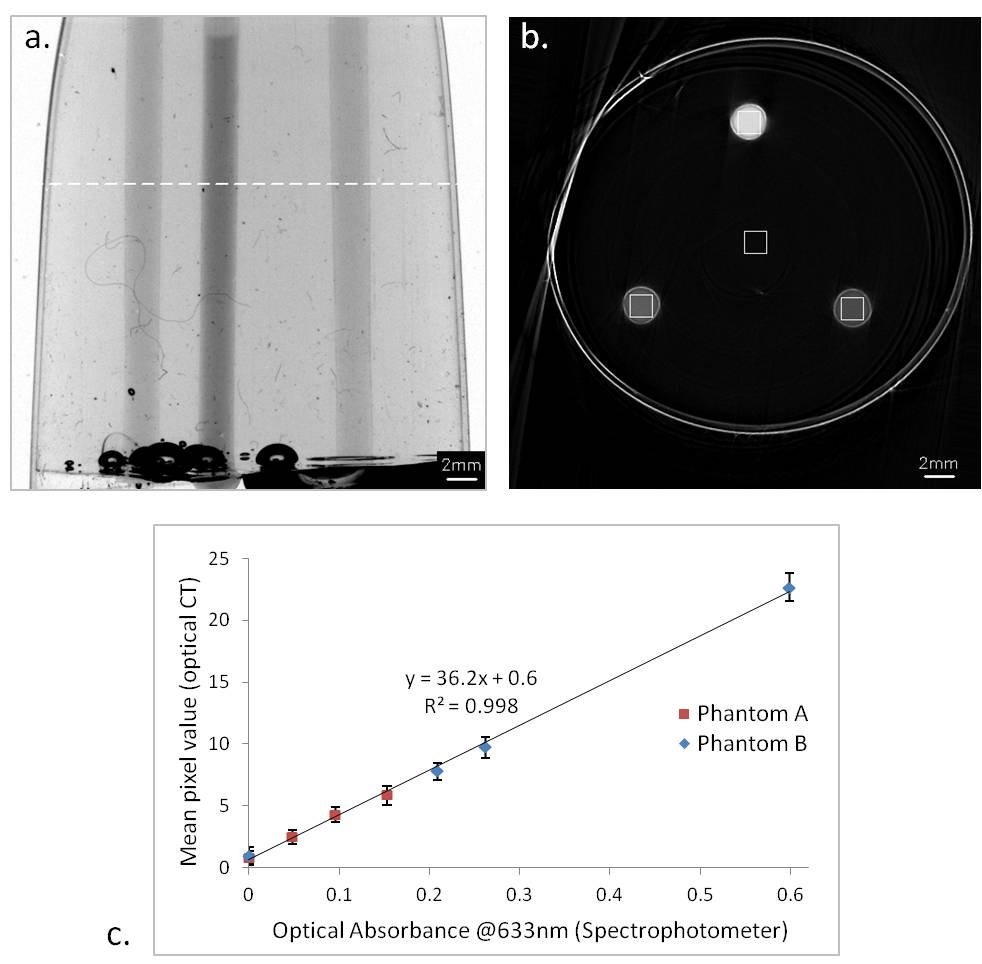
\includegraphics[width=1\textwidth]{meth_img/EB_rod_new.jpg}
		\caption{a. An optical CT projection image of a gelatin phantom containing `finger' inclusions of different concentrations of Evans blue-dyed gel. b. A reconstructed slice through the phantom in the axial position marked by the dashed line in (a). Regions of Interest (ROIs) mark where the mean pixel value was calculated for each finger and the clear gelatin. The double ring artefact is due to refractive index mismatch between gel and the Teflon FEP container, and also between the Teflon and 4.5\% saline solution matching liquid. c. Plot of absorbance of Evans Blue-doped gel measured with a Spectrophotometer against mean pixel value of different regions on reconstructed optical CT images. Two phantoms were measured  with all  variables constant between readings.}
		\label{fig:fingerphantoms_roi_EB}
	\end{figure}
	



We expected that once the absorbance is too high the system response will drop off non-linearly due to a lack of photons. This was demonstrated with a PRESAGE sample containing very large doses of radiation. Show graph of L3?






\subsection{Spatial resolution}

\label{subsubsec:MTF}

Understanding the spatial resolution response of the optical CT system is very important for acquiring high-quality, quantitative images. 
Previous publications noted a reduction of optical CT image contrast of small features as the feature size approaches the resolution. \cite{doranultra-high2013} This effect is evident even when the feature size is several times the nominal spatial resolution and leads to non-linear response to optical absorbance. Therefore, the limits of spatial resolution of the system must be carefully characterised before we can be confident that measurements are quantitative. 

There are many factors which can affect optical CT resolution (see theory section?). There is an added complexity when imaging extended objects as standard microscope lenses are designed to image a thin sample at the focal plane. For optical CT the spatial resolution either side of the focal plane is important as ideally the entire sample should be in focus at all times (see Figure~\ref{fig:idealdof}). The distance over which the focus is `acceptable' is known as the depth-of-field (DOF).

\begin{figure}[H]
	\centering
	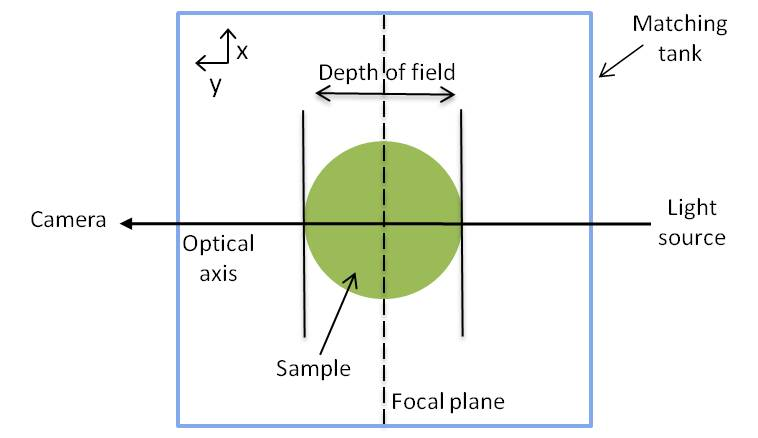
\includegraphics[width=0.9\linewidth]{meth_img/ideal_dof_diagram}
	\caption{Schematic of the optical CT system geometry showing the ideal positions of the focal plane and depth-of-field.}
	\label{fig:idealdof}
\end{figure}

Our optical system consists of components from a modular microscope system. This includes a zoom lens, giving variable magnification settings, and a variable aperture which controls the DOF of the system. 
The aperture size can determine the overall acceptance angle of the optical system, $\theta$, which in turn affects the numerical aperture (NA), defined as $N_A = n \sin{\theta}$.  A system with high NA results in high resolution, $\Delta x$ (Equation~\ref{eqn:airy}). However, such a system has a small DOF due to the inverse relationship between DOF and NA (Equation~\ref{eqn:dof}).
\begin{equation}
\Delta x =  \frac{0.61 n\lambda}{N_A}
\label{eqn:airy}
\end{equation}
\begin{equation}
\mathrm{d_{DOF}} = n_{bath}\left( \frac{n\lambda}{N_{A}^2}+\frac{ne}{MN_{A}} \right) = \frac{n_{bath}}{0.61n\lambda}\left( \Delta x^2 + \frac{n e}{M}\Delta x \right)
\label{eqn:dof}
\end{equation}
where $n$, the refractive index of the medium around the lens, $n_{bath}$ the refractive index of the medium surrounding the sample, $M$ the lateral magnification of the system, $e$ the pixel size of the camera and $\lambda$, the wavelength of light.





To investigate the effect of changing the NA of our system we measured the modulation transfer function (MTF) for a range of positions along the optical axis. Five different NA values were evaluated, corresponding to the five reproducible aperture size settings on the lens system, labelled as A=1 to A=5, with A=1 being the smallest aperture and A=5 being the fully open aperture setting. 

The modulation transfer function (MTF) characterises the resolution of a system by measuring how different spatial frequencies are transmitted.
It is the Fourier transform of the Point Spread Function (PSF), giving a more comprehensive description of an optical system than quoting a single  resolution value. There are various methods of measuring the MTF including simulating a point source or measuring the response to a sinusoidal pattern. These methods require test objects accurate to sub-pixel distances. 
It is much easier to manufacture an accurate  sharp edge rather than  a point source or slit. It has been shown that the MTF can be calculated analytically from the Edge Spread Function (ESF) as follows,
\begin{equation}
\mathrm{MTF}(f) = \mathscr{F}\left[\mathrm{LSF}(x)\right] = \mathscr{F}\left[\frac{d}{dx}\mathrm{ESF}(x)\right]
\end{equation}
where $f$ is spatial frequency, $x$ is displacement and LSF is the Line Spread Function given by the profile of a slit source. \cite{Boone:1986}

Any noise in the data is amplified  through the derivative and Fourier transform. Therefore, following the method of Boone \textit{et al.},   the MTF was calculated directly from the fit parameters of a function  fitted directly to measured ESF data. \cite{Boone:1994} Analysis was carried out in IDL  using curve fitting function `\textit{mpfit}'.  \cite{Markwardt2009mpfit}

A knife edge was positioned at the focal plane and 50 projection images of matrix size $2048\times 2048$ were acquired and averaged to improve the signal-to-noise ratio (SNR). The knife edge was moved in steps of 0.1mm away from the focal plane in both directions along the optical axis.  Images were acquired over a distance of 0.5mm in each direction giving a total distance of 1mm, the same as the FOV of each projection image. This was repeated for each aperture setting of the microscope lens.


Plotting the MTF at each position along the optical axis as an image, the DOF is visualised in a similar manner to  \cite{chenincorporation2012}. The maximum resolution for each NA was taken as the largest spatial frequency with continuous MTF values over 0.1 over some y-range, being the DOF for that resolution.


The MTF was calculated from ESF data, as seen in Figure~\ref{fig:MTFtarget},  for a range of magnifications, pixel binning and LED voltages. The results  in Figures~\ref{fig:MTF_50}  show that system response varies significantly with these variables as is expected. Magnifcations of 0.8, 1 and 8 were tested to demonstrate the worst,  standard and best conditions for imaging respectively.





The MTF was calculated from the ESF, measured across the centre of the knife-edge images, according to equation ? for each position along the optical axis and for each NA value. The MTF was represented by a grey level in a 2-D image in which the horizontal coordinate corresponds to spatial frequency, up to the desired 100mm$^{-1}$ (equivalent to a $10\mu$m line-pair), and the vertical coordinate corresponds to position along the optical axis. This allows visualisation of the DOF for each of the different NA values.
The maximum resolution and corresponding DOF were measured for each NA setting. The maximum resolution was defined as the largest spatial frequency with an MTF above 10\% at the focal plane. The DOF for this frequency was defined as the distance along the optical axis for which this spatial frequency had an MTF above 10\%.  



	\begin{figure}[H]
		\centering
		\subfigure[`Knife-Edge' Target]{\label{subfig:MTFtarget}
			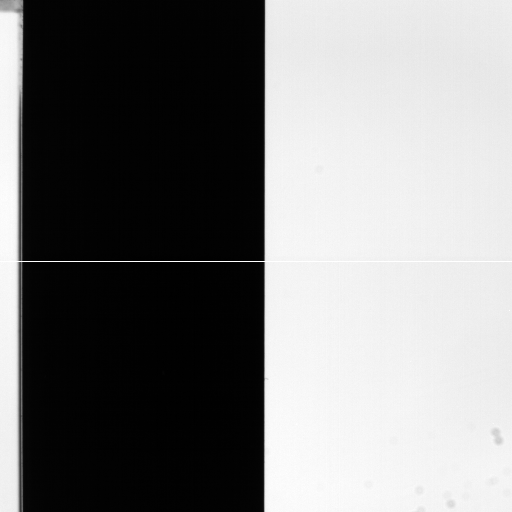
\includegraphics[width=0.3\linewidth]{meth_img/MTF3_targetimage.png}}
		\subfigure[Edge spread function from image \ref{subfig:MTFtarget}]{\label{subfig:ESF}
			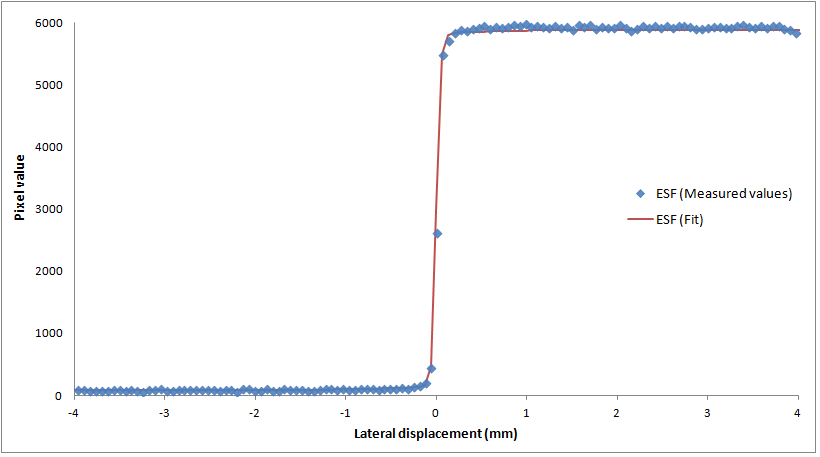
\includegraphics[width=0.55\textwidth]{meth_img/croppedESF_MTF3.png}}
		\caption{Image of a rectangular metal target with a straight edge which  approximates a `Knife' edge for the measurement of the Edge Spread Function (ESF, \ref{subfig:ESF}). The pixel row across which the ESF is measured is marked on the image. This data was cropped to give 300 points centred on the edge to allow a curve to be fitted to the data  accurately.  Pixel size was measured  allowing the pixel values to be plotted against displacement. The point of zero displacement was set at the edge for convenience in fitting a curve to the data.  The MTF is calculated directly from the ESF via  fit parameters. }
		\label{fig:MTFtarget}
	\end{figure}

	\begin{figure}[H]
		\centering
		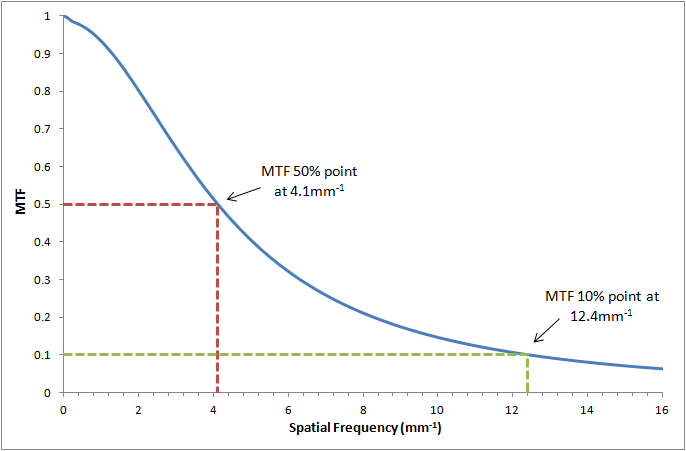
\includegraphics[width = 0.7\textwidth]{meth_img/MTF_50_graph.png}
		\caption{MTF vs spatial frequency for the case of M=1, 4x4 binning to 512x512 pixels and  LED voltage set to just below camera saturation levels, representing the imaging conditions  for most phantom images in this report. The 50\% cut-off point for the MTF, a value commonly quoted as giving the best focus is found to be $4.1mm^{-1}$. The 10\% MTF value is 12.4$mm^{-1}$ and in general this value indicates the highest  frequency that can be resolved by the system. This implies that features smaller than $40\mu m$ will not be resolved at this magnification and binning.}
		\label{fig:MTF_50}
	\end{figure}








The observed DOF and resolution results are shown in Table... and images of MTF against optical axis position are shown in Figure REF.
It is apparent that for low NA, there is a constant, low resolution across the entire FOV whereas at high NA there is a small region of high-resolution with other areas being defocused. 
%NA values in between show a sharp drop-off of DOF.





These results indicate that aperture settings must be chosen carefully for each imaging application. For most cases a constant resolution across the FOV is desirable, therefore A=1 is appropriate. For some cases, it may be desirable to have very high resolution in a small area around the centre of rotation in which case a higher aperture setting may be appropriate. However, positioning of the focal plane is very sensitive,  illustrated through the use of a `point' object test phantom containing $5\mu $m beads (Figure REF), it is apparent that the focal plane is not at the centre of the object. It is possible to attach this  bead phantom to the bottom of other samples which gives us the ability to quantify  how the resolution changes over the FOV. 



	



Ideally the DOF of projection images should be larger than or equal to the sample size, as demonstrated in Figure~\ref{fig:idealdof}. However, there is a trade-off between DOF and resolution,  $\Delta x$, given by \cite{inoue1997video} as follows,
\begin{equation}
DOF = \frac{n_{bath}}{0.61 n \lambda} \big(\Delta x^2 + \frac{ne}{M_{lat}} \Delta x \big)
\label{eqn:1DOF}
\end{equation}
where, $n_{bath}$ is the refractive index of the medium surrounding the sample, $n$ is the refractive index of the medium around the lens, $\lambda$ is the wavelength of light, $e$ is the pixel size of the camera and $M_{lat}$ is the lateral magnification of the system. The DOF of the system can be adjusted by adjusting the overall acceptance angle of the system, $\theta$, which in turn controls the numerical aperture (NA) and this is inversely proportional to the resolution, 
\begin{equation}
NA = n \sin \theta = \frac{0.61n\lambda}{\Delta x}
\label{eqn:2NA}
\end{equation}



	\begin{figure}[H]
		\centering
		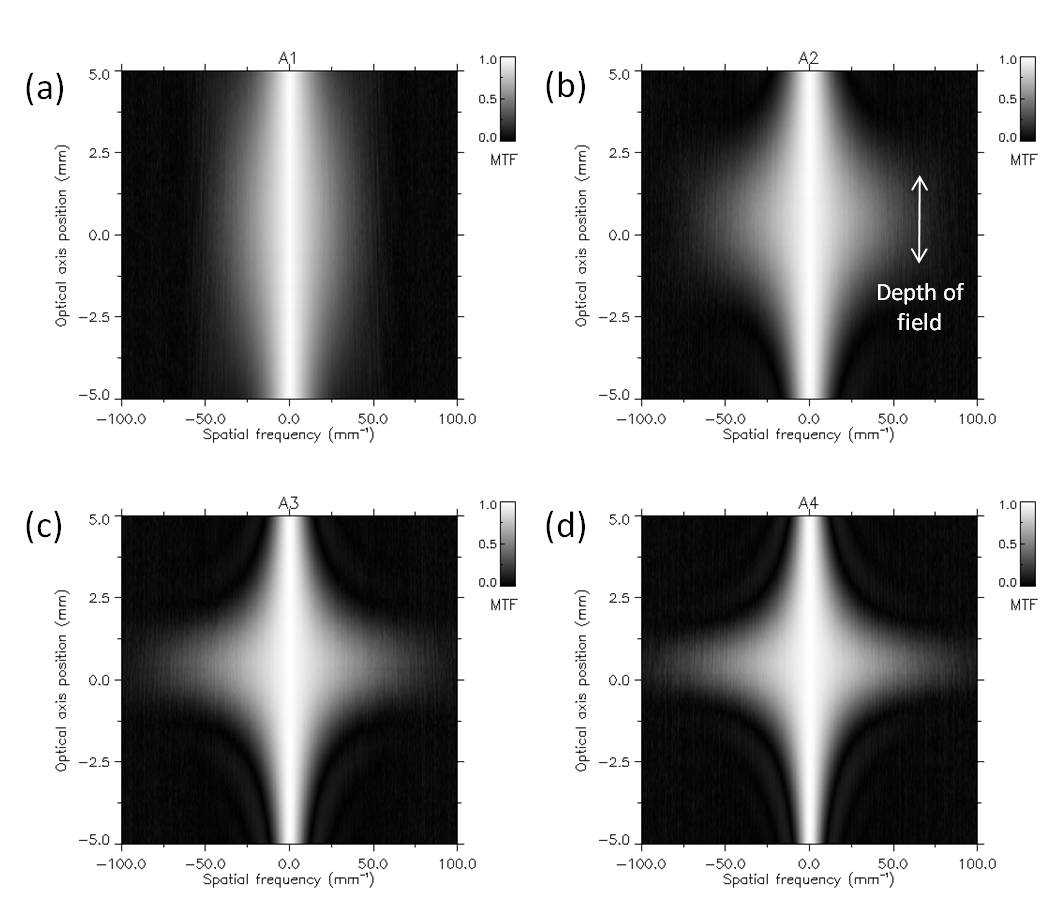
\includegraphics[width=0.9\linewidth]{mrt_img/mrt_Fig6}
		\caption{Measurements of the modulation transfer function (MTF) along the optical axis for different numerical aperture (NA) settings of the system, (a) A1 (b) A2 (c) A3 (d) A4. This allows visualisation of the depth-of-field (DOF).}
		\label{fig:MTFDOF}
	\end{figure}
	
	\begin{table}[H]
		\centering
		\begin{tabular}{ p{2.5cm}  p{3.5cm} p{4.5cm}  }
			\hline
			\textbf{NA setting} & \textbf{Resolution ($\mu$m)} &\textbf{Depth of field (mm)}  \\ \hline
			A1  & $21.5 \pm 0.5$ & $9.3 \pm 0.4$ \\ %\hline
			A2  & $13.7 \pm 0.1$ & $2.4 \pm 0.2$ \\ %\hline
			A3  & $12.0 \pm 0.2$ & $1.6 \pm 0.2$ \\ %\hline
			A4  & $10.1 \pm 0.2$ & $0.6 \pm 0.1$ \\ %\hline
			A5  & $9.7 \pm 0.2$ & $0.4 \pm 0.1$ \\ \hline		
		\end{tabular}
		\caption{Maximum resolution and corresponding depth-of-fields for different NA settings on the optical CT system. The uncertainties reflect noise in the modulation transfer function (MTF)  measurements.}
		\label{table:DOFNA}
	\end{table}



These measurements were all taken in `projection' space and do not take into account the effect of the reconstruction process on resolution. 

Bead phantom construction. A=5, m=8, sum 50 slices to get good visualisation

\begin{figure}{H}
\centering
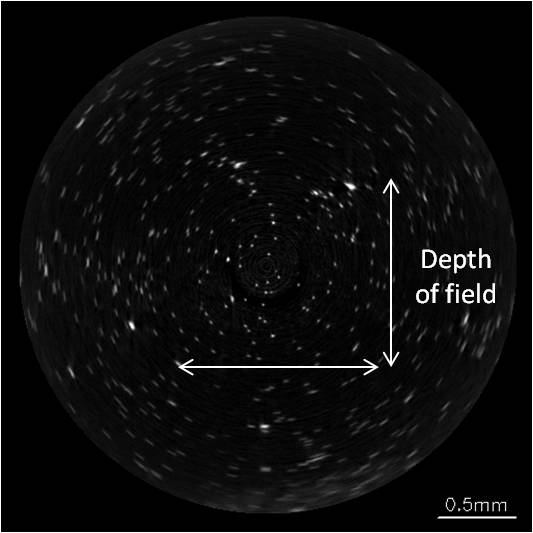
\includegraphics[width=0.7\linewidth]{meth_img/bead_DOF_d2_res_test_1_10_15_scan5.jpg}
\caption{Bead imgs}
\label{fig:bead_DOF}
\end{figure}





















